\documentclass[journal]{IEEEtran}
\usepackage{graphicx} % Required for inserting images
\usepackage{hyperref}

\begin{document}

\begin{center}
   \Large Garden Automated Rain/Daylight Executed by Near-Infrared Sensing \break

   \large Nicholas Chitty, Brendan College, Scott Pierce, Justin Pham-Trinh \break

   \large University of Central Florida, Dept. of Electrical and Computer Engineering, Orlando,
   Florida, 32816-2450
\end{center}

\begin{abstract}
   This paper will show the application of near infrared spectroscopy 
and how it can measure electromagnetic waves from the emission of soil. Near infrared spectroscopy 
is an absorption spectroscopy method that can help determine the chemical composition of a 
substance through the radiation the substance gives off. Soil itself is a mixture of organic and 
inorganic substances that all together directly contribute to a garden’s environment. We are 
starting with soil with unknown qualities, so comparisons will be made between our soil and soil 
of known qualities to match and ensure that our plant is in a healthy and suitable environment. 
\end{abstract}

\section{Introduction}
\IEEEPARstart{I}{n} the past year, we have seen a great increase in remote sensing, wireless 
communication, API integration, and so much more. All of which have been made more available and 
economical. The internet has also seen its share of ``DIY" projects and its continuing growth.

In the agriculture industry, there have been new advancements in technology with high performance 
water distribution, network communication, and remote sensing. This research is intended to advance
the field by producing a system that can maintain a suitable environment for a plant to grow. In the 
environment, there will be sensors that will help modify the conditions within the environment. In 
addition to this system, it will feature a web interface for notifications and the ability for the 
user to set settings.

Monitoring soil isn't always the most fun or the easiest task, because things could get dirty or we 
might forget about our plant. This project will feature an on-the-rise technology in the form of a 
spectrophotometer. Smart systems nowadays are big learning machines that are constantly aware of its 
surroundings. For a smart agricultural system, it would need to determine variables such as moisture 
levels, nutrient content, pH levels, and so much more. This paper will introduce near infrared 
spectroscopy as another method to soil sensing that may prove to be more beneficial over traditional 
products or techniques.

This project will also present other fields such as system controls, power, and web, all to provide 
a "set it and forget it" home gardening experience. A home gardening experience where the garden bed 
can communicate with the user and the user can provide instruction of what to do, but also at the 
core, this is a microcontroller project that anybody can do with just slight knowledge and understanding
of digital communications. Like any smart device too, the internet plays an important role in making 
this as hands-off as it can be. There are many different communication protocols such as Bluetooth, 
Zigbee, Thread, and even short-range/long-range protocol. For this project we decided to go with WiFi 
because of its decreased bandwidth and that we aren't expecting to produce or receive large amounts 
of data. 

An important aspect to a lot of devices as well is data storage and web usage. This is important so 
that we can look back on previous information and make observations and conclusions. With our 
microcontroller, the web system is going to communicate with it through transmission control protocol.
Transmission control protocol is a standard on how to establish and maintain a network connection to 
exchange data. The web system will also have 16gb database to store data and have the ability to support 
multiple garden beds in a scaled solution. As mentioned before, the web system will have a feature to 
allow the user to set settings but also read the data that is stored. Lastly, an important factor to 
any garden is the weather and knowing when it might be cold, hot, or even rain outside. As a part of 
our web system, it will communicate using HTTP requests with a weather service to receive updates on 
the weather.

Solar power has been a growing source of energy for the past years and still continues to be with new 
developments and breakthroughs with solar technology. A lot of systems nowadays are solar powered but 
these products are not constantly in use, they have to turn of eventually. When the product is off the 
solar panel can still collect energy which is stored in a battery for conservation. In this paper, we 
will demonstrate our system running independently, battery powered but charged through solar panels.

In all, this paper will present how near infrared spectroscopy can be used to monitor a plant's environment 
and notify users with information of its health. Generating and guiding electromagnetic waves into a 
housing, scanning the substance, and then converting this optical power into a voltage that can be 
read and analyzed. It is then the microcontroller will communicate with the web system, storing the 
information and deciding on if anything needs to be done and notifying the user. 
\subsection{Goals} \label{sec:goals}
The following are the goals the team set for themselves with this project. Starting with non-
negotiable goals:
\begin{enumerate}
   \item A spectrometer that operates in the 400nm to 1700nm band with a spectral resolution less
         than 50nm and signal-to-noise ratio greater than 2.
   \item The ability to automatically feed water into the garden bed.
   \item Serve data to the user.
\end{enumerate}
Moving on, the team had goals they hoped to accomplish:
\begin{enumerate}
   \item Power the garden bed completely from solar and battery power.
   \item Serve data to the user via a website.
\end{enumerate}
\section{High-Level Design}
Based on the goals listed in \autoref{sec:goals} this section will discuss the high-level thought
process the team undertook in achieving those goals.
\begin{figure}[H]
    \centering
    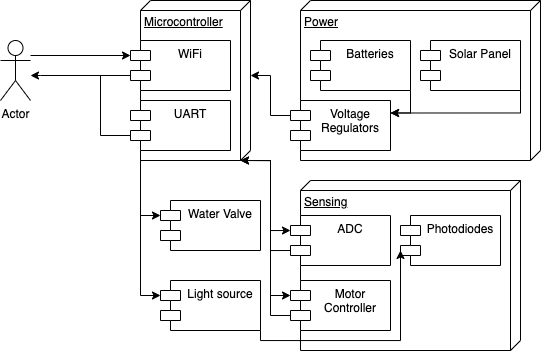
\includegraphics[width=\textwidth]{images/Flowchart.png}
    \label{fig:flowchart}
    \caption{The large systems and their interfaces and submodules}
\end{figure}
\subsection{Spectrometer} 
In most instances, spectrometers are designed using charged couple devices in an array which some
component such as a prism or diffraction grating will shine upon breaking the source into its
components. This approach would be prohibitively expensive for such a consumer-oriented garden
bed. The solution was to use either a photodiode or photoresistor to measure the magnitude of the
of optical power in a given area. This sensor could be moved in order to give the effect of shining
the source on an array with the only major downside being the duration needed to scan. 
\section{Major Components} \label{sec:major-components}
The components found in this section make up the logical boundaries between systems and their
subsystems. 
\section{Hardare Detail}
In \autoref{sec:major-components}, a high level overview of components and features were given. This
section will discuss the implementation details of the chosen components.
\section{Software Detail}
The microntroller serves as the glue holding this design together. In this section the means of
integrating the various subsystems via software will be discussed.
\end{document}